\documentclass{article}
\usepackage[margin=2cm]{geometry}
\usepackage{graphicx}
\usepackage[pages=some]{background}
\usepackage{titling}
\usepackage{tabularx}
\usepackage{tikz}
\usepackage{forest}
\usepackage{float}

\forestset{
  my box/.style={
    draw,
    rectangle,
    rounded corners,
    fill=gray!20,
    inner sep=6pt,
    minimum width=3cm % Adjust the width as needed
  }
}


\geometry{a4paper}

\backgroundsetup{
    scale=1,
    angle=0,
    opacity=1,
    contents={%
        
\includegraphics[width=\paperwidth,height=\paperheight]{institution_logo.jpg}
    }
}

\newcommand{\subtitle}[1]{
    \posttitle{
        \par\end{center}
        \begin{center}\large#1\end{center}
        \vskip0.5em}
}

\title{ME-421}
\author{Md. Hasibul Islam}
\subtitle{FLUID MACHINERY}

\begin{document}
\begin{titlepage}
    \centering
    
    {\Huge\bfseries\maketitle}
    \textbf{Mohammad Ali Sir} \\
    \vspace{2cm}
    
\includegraphics[width=8cm]{institution_logo.jpg}
    \vfill
    \vspace*{2cm}
\end{titlepage}

\tableofcontents
\pagebreak
\section{Lecture 01: Introduction} 
\hfill Date: 03/06/2023
\subsection*{Booklist}

\textbf{Hydraulic Machines through worked out problems}

\hfill Published by BUET


\section{Lecture 2: Principles of Hydraulic Machinery}
\hfill Date: 05/06/2023

\subsection{Dynamic Action of Fluid}

When a stream of fluid enters a machine, it generally follows a specific direction. However, in order to alter its velocity, either in magnitude or direction, a force must be applied to the fluid. This force, exerted by the motion of the fluid, is referred to as dynamic force. The power of the machine is determined by the dynamic force generated by the flowing fluid, which arises due to the change in momentum.

Momentum can exist in linear or angular form, with angular momentum being the moment of linear momentum. The force is the rate of change of linear momentum, while torque is the rate of change of angular momentum. According to Newton's second law, the rate of change of momentum is proportional to the applied force and occurs in the direction of the force. Specifically, if the resultant external force in the $x$-direction is $F_x$, the mass of the fluid is $m$, the velocity of the fluid is $v_x$, and the change in velocity over time $dt$ is $dv_x$, then:
\\

The change in momentum = $mdv_x$,

And the rate of change of momentum  $= m \frac{dv_x}{dt}$
\begin{equation}
F_x = m \frac{dv_x}{dt} \label{eq:eq1}
\end{equation}

$eq^n$ (\ref{eq:eq1}) is knows as linear momentum $eq^n$.

This $eq^n$ may be wriiten as -
\begin{equation}
F_x dt = mdv_x \label{eq:eq2}
\end{equation}

This $eq^n$ is known as impulse momentum $eq^n$.

For a control volume with fluid entering in uniform velocity $v_{x_{1}}$, and leaving after time $t$ within uniform velocity $v_{x_{2}}$, then according to $eq^n$ (\ref{eq:eq2}),
\begin{equation}
	F_x = \frac{m}{t} (v_{x_{2}}-v_{x_{1}}) \label{eq:eq3}
\end{equation}

Again, $$\frac{m}{t}=\rho Q$$
\begin{equation}
	\Rightarrow F_x = \rho Q (v_{x_{2}}-v_{x_{1}}) \label{eq:eq4}
\end{equation}

Dynamic force exerted by fluid jet on stationary flat plate - 

\subsubsection{Plate normal to jet:}
A fluid jet is issued from a nozzle and strike a flat plate with a velocity $v$. The plate is held stationary at perpendicular to the centerline of the jet. Let,

\begin{center}

$Q \longrightarrow $  Volumetric flow rate\\
$\rho Q \longrightarrow$ Mass flow rate
\end{center}

Dynamic force on the fluid by the plate:
\\
Applying $eq^n$ \ref{eq:eq4}, 
$$F_x = \rho Q (v_{x_{2}} - v_{x_{1}}) $$
$$\Rightarrow -F_x = \rho Q (0-v)$$
\begin{equation}
	\Rightarrow F_x = \rho Q v \label{eq:eq5}
\end{equation}
\begin{equation}
	\Rightarrow F_x = \frac{\gamma}{g} Q v \label{eq:eq6}
\end{equation}

\begin{figure}[H]
  \centering
  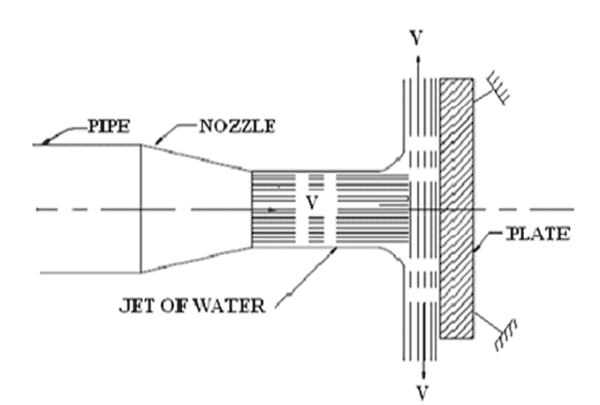
\includegraphics[width=0.75\textwidth]{img/flat_plate.png}
  \caption{Plate normal to jet.}
  \label{fig:Plate normal to jet}
\end{figure}

If $a$ is the area of jet,
$$F_x = \frac{\rho}{g} a v  v$$
\begin{equation}
	\textcolor{red}{\Rightarrow F_x = \frac{\rho}{g} a v^2} \label{eq:eq7}
\end{equation}

\subsubsection{Inclined Plate}
\begin{figure}[H]
  \centering
  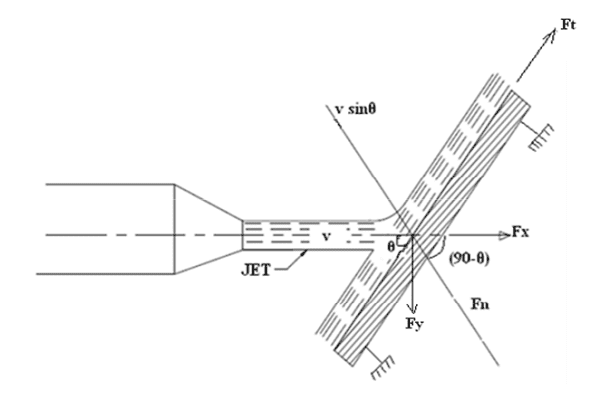
\includegraphics[width=0.75\textwidth]{img/inclined_plate.png}
  \caption{Plate inclined to jet.}
  \label{fig:Plate inclined to jet}
\end{figure}
\vspace{0.25cm}

$$F = F_n = \rho Q v sin\theta $$
Again, $$F_x = F sin\theta$$
$$= (\rho Q v sin \theta) sin \theta $$
\begin{equation}
	\textcolor{red}{F_x = \rho Q v sin^2 \theta} \label{eq:eq8}
\end{equation}
\\
And, $$F_y = F cos\theta$$
\begin{equation}
	\textcolor{red}{\Rightarrow F_y = \rho Q v sin\theta cos\theta} \label{eq:eq9}
\end{equation}
\vspace{0.25cm}
\paragraph*{Determine of division of flows:}
Let $F_s$ ($F_t$ in fig. \ref{fig:Plate inclined to jet}) be the force along the inclined surface of plate and $Q_1$ and $Q_2$ are quantities of flow along the surface. As there is no change in elevation of pressure before and after impact, the magnitude velocity leaving the plate will remain the same. \\
\\
since no force is exerted on the fluid by the plate in "S" direction, then,
\begin{equation}
	F_s = 0 = \rho Q V cos\theta \label{eq:eq10}
\end{equation}
Again, 
\begin{equation}
	\rho Q_1 v - \rho Q_2 v = 0 \label{eq:eq11}
\end{equation}

From $eq^n$ (10) \& (11),
$$\rho Q v cos\theta = \rho Q_1 v - \rho Q_2 v $$
\begin{equation}
	\Rightarrow Q cos\theta = Q_1 - Q_2 \label{eq:eq12}
\end{equation}

From continuity $eq^n$, 
\begin{equation}
	Q_1 + Q_2 = Q \label{eq:eq13}
\end{equation}

From $eq^n$ (12) \& (13),

\fbox{\begin{minipage}{0.5\textwidth}
\textcolor{red}{$$ Q_1 = \frac{1}{2} Q (1+cos\theta)$$
$$ Q_2 = \frac{1}{2} Q (1-cos\theta) $$}
\end{minipage}}
\pagebreak

\end{document}
